\subsection{Logical View}

I logical view for user, er det kun user storien "Indstil profilbillede og personligt tema", som skal implementeres. På baggrund af det meget begrænsede funktionalitet som skal implementeres for user, laves der et kortfattet klassediagram, som kan ses i \ref{fig:UserController_Class}

\begin{figure}[H]
    \centering
    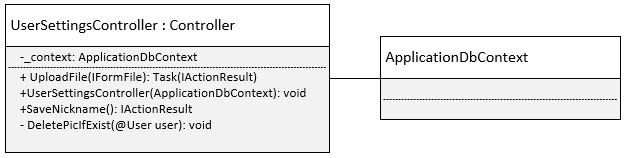
\includegraphics[width=0.9\linewidth]{09_Arkitektur/User/Images/US_Class.JPG}
    \caption{UserController klassediagram: Der ses at klassen har en constructor, som initierer ApplicationDbContexten. Derudover er der en UploadFile action, som er en HttpPost, der modtager en IFormFile, ud fra denne IFormFile kan der udtrækkes profilbilledets data, og skrives ind i projektet, og filstien gemmes i User entiteten.}
    \label{fig:UserController_Class}
\end{figure}

\noindent Temaet er blevet besluttet at blive bygget i \_layout viewet som en drop-down knap, hvor temamulighederne dukket op. Funktionerne som bliver kaldt på disse knapper, bliver skrevet i JavaScript, og fremgår derfor ikke i klassediagrammet.